\chapter{Introduction}
Artificial intelligence is playing more prominent role in our daily lives by demonstrating human intelligence by machines, especially computer systems. The field includes learning, reasoning and self-correction. These can be described as the acquisition of information and rules for using the information, using the rules to reach approximate or definite conclusions. It has become more important to make machines able to communicate through natural language with human or among machines themselves. Learning algorithms for natural language understanding in language translation, reading comprehension have progressed at a rate in recent years that never done before, but that lack ultimate aspects of how humans understand and produce natural language. Mainly humans develop language understanding and producing by being embodied in an environment which they can realize and interact with other humans~\cite{DBLP:journals/corr/abs-1807-03367}.

In many tasks understanding compositional language in context is very complex. Reasoning about sets of objects, quantities, comparisons and spatial relations are required in visual question answering and robot instruction systems. Robust language understanding is required when instructing assembly-line or home assistance robots to manipulate objects in random environments. And this is only partially addressed by existing datasets~\cite{Suhr2017ACO}.

Since the early days of artificial intelligence, the problem of interpreting instructions written in natural language has been widely studied. The automation of tasks that currently require human participation would be enabled by mapping instructions to a sequence of executable actions~\cite{RL}.



``Natural Language" refers to a human language that is used for everyday communication by humans; languages like English, Bengali or Portuguese as distinct from the typically artificial command. Artificial language like programming language and mathematical transcripts, natural languages have evolved over generations, and hard to keep down with explicit rules. NLP based technologies are becoming increasingly widespread. For example, phones and handheld computers support text suggestion and handwriting recognition;web search engines provide access to information locked up in noisy text data;machine translation allows us to recover written texts in different language and read them in another language; text analysis enables us to classify sentiment in different reviews or blogs post. By providing a more natural human-machine interfaces and more sophisticated access to stored data, a central role is played by language processing in multilingual information society~\cite{NLPbook}.

It is straightforward to induce our hands on countless words of text. What will we have a tendency to do with it, forward we are able to write some easy programs? We're all terribly accustomed to text, since we have a tendency to scan and write it on a daily basis. Here we'll treat text as data for the programs we have a tendency to write, programs that manipulate and analyze it in an exceedingly type of attention-grabbing ways.
\section{Robot Navigation}
Navigation refers to the strategy of crucial aspects like position, speed, and direction throughout travel. within the pre-modern era, direction associate degreed position were determined mistreatment an measuring instrument, a compass, and a map; these square measure currently thought of primitive kinds of navigation. As a results of fashionable developments in science and technology, precise positions and speeds square measure determined mistreatment instrumentation like artificial satellites, international navigation satellite system (GNSS), direction systems (INS), etc~\cite{NAV}.

\section{Automatic Natural Language Understanding}
At a strictly sensible level, we tend to all want facilitate to navigate the universe of knowledge fast up in text on the net. Search engines are crucial to the expansion and recognition of the net, however have some shortcomings. It takes talent, knowledge, and a few luck, to extract answers to such queries as: \emph{What tourist sites can I visit between Philadelphia and Pittsburgh on a limited budget? What do experts say about digital SLR cameras? What predictions about the steel market were made by credible commentators in the past week?} Getting a machine to answer them automatically involves a variety of language process tasks, as well as info extraction, inference, and account, and would want to be dispensed on a scale and with grade of hardiness that's still on the far side our current capabilities.

On a a lot of philosophical level, a long-standing challenge at intervals AI has been to create intelligent machines, and a serious a part of intelligent behavior is knowing language. for several years this goal has been seen as too troublesome. However, as information science technologies become a lot of mature, and sturdy strategies for analyzing unrestricted text become a lot of widespread, the prospect of language understanding has re-emerged as a plausible goal~\cite{NLPbook}.

In this section we tend to describe some language understanding technologies, to allow a way of the attention-grabbing challenges that area unit associated with NLP.
\subsection{Word Sense Disambiguation:}
In word meaning disambiguation we wish to figure out that sense of a word was supposed in an exceedingly given context. Contemplate the ambiguous words serve and dish:

\begin{enumerate}[a.]
    \item serve: help with food or drink; hold an office; put ball into play
    \item dish: plate; course of a meal; communications device    
\end{enumerate}
In a sentence containing the phrase: he served the dish, square measure able to notice that each serve and dish are being employed with their food meanings. It's unlikely that the subject of dialogue shifted from sports to crockery within the space of 3 words. This might force us to create outre pictures, sort of a professional tennis player removing his or her frustrations on a china tea-set arranged out beside the court. In alternative words, we have a tendency to automatically clear up words exploitation context, exploiting the straightforward incontrovertible fact that close words have closely connected meanings. As another example of this discourse result, take into account the word by, that has many meanings, e.g.: the book by Russel (agentive -- Russel was the author of the book); the match by the stove (locative -- the stove is where the match is); and submit by Saturday (temporal -- Saturday is the time of the submission). Observe in (c) that the meaning of the italicized word helps us interpret the meaning of by.

\begin{enumerate}[a.]
    \item The lost women were found by the searchers (agentive)
    \item The lost women were found by the mountain (locative)
    \item The lost women were found by the afternoon (temporal)    
\end{enumerate}

\subsection{Pronoun Resolution}
A deeper reasonably language understanding is to figure out "who did what to whom" — i.e., to observe the subjects and objects of verbs. You learnt to try and do this in grammar school, however it's tougher than you may assume. In the sentence the thieves stole the paintings it's simple to detect who performed the stealing action. Consider 3 doable following sentences in (c), and check out to see what was sold, caught, and found (one case is ambiguous).
\begin{enumerate}[a.]
    \item The thieves stole the paintings. They were subsequently sold.
    \item The thieves stole the paintings. They were subsequently caught.
    \item The thieves stole the paintings. They were subsequently found.
\end{enumerate}
Answering this question involves looking for the preposition of the pronoun they, either thieves or paintings. One of the calculation techniques to address this problem includes anaphora resolution -- identifying what a pronoun or noun phrase means -- and labeling semantic role -- identifying the relation between a noun phrase and the verb (as agent, patient, instrument, and so on).

\subsection{Generating Language Output}
If we are able to automatically solve such issues of language understanding, we are going to solve the tasks that involve generating language output, like responding to a question and translating language from one form to another. In the initial case, a machine ought to be ready to answer a user's query regarding to text collection.

\begin{enumerate}[a.]
    \item Text: ... The thieves stole the paintings. They were subsequently sold. ...
    \item Human: Who or what was sold?
    \item Machine: The paintings.
\end{enumerate}
The answer of machine proves that it has correctly worked out that \emph{they} doesn't refer to the thieves but to paintings. 

In the second case, the machine should be able to translate the text into another language, accurately conveying the meaning of the original text. In translating the example text into French, we are forced to choose the gender of the pronoun in the second sentence: \emph{ils} (masculine) if the thieves are found, and \emph{elles} (feminine) if the paintings are found. Correct translation actually depends on correct understanding of the pronoun.
\begin{enumerate}[a.]
    \item The thieves stole the paintings. They were subsequently found.
    \item Les voleurs ont volé les peintures. Ils ont été trouvés plus tard. (the thieves)
    \item Les voleurs ont volé les peintures. Elles ont été trouvées plus tard. (the paintings)
\end{enumerate}
In these examples, the definition of a word, the subject of verbs, and the pronoun sit-in are the steps of the meaning of a sentence that we hope to be able to understand.

\subsection{Spoken Dialog Systems}
In the study of past of artificial intelligence, the main measure of intelligence has been a linguistic, Turing test: if a dialog system, responding to a user's text input, can perform so naturally that we can't differentiate it from human-generated reactions. Can't i? On the contrary, today's commercial dialog systems are very limited but still perform useful functions in short-term domains, as we can see here:\\
S: How may I help you?\\
U: Deliver some food from the list to Shahidullah Hall after buying these from TSC.\\
S: Buying food from TSC first and then deliver these to Shahidullah Hall?\\
U: Yes.\\

We could not ask the machine to produce driving directions or details of nearby restaurants unless the specified info had already been hold on and appropriate question-answer pairs had been incorporated into the language processing system.

Observe that this system understands the sequence of working plan based on the instruction: the user tells an instruction in complex way and the system correctly determines from this that the user wants to deliver some food but it needs to buy these foods first. This assumption seems so obvious that you probably didn't notice that it was trained, yet a natural language system needs to be completed with this skill to communicate naturally. WIthout it, when asked \emph{Deliver some food from the list to Shahidullah Hall after buying these from TSC.}, a system might plan to deliver first and to buy food from TSC.
Usually contextual assumptions and business logic is used in commercial dialogue systems to ensure that a user can request or provide information that pays for specific applications.

\begin{figure}
    \centering
    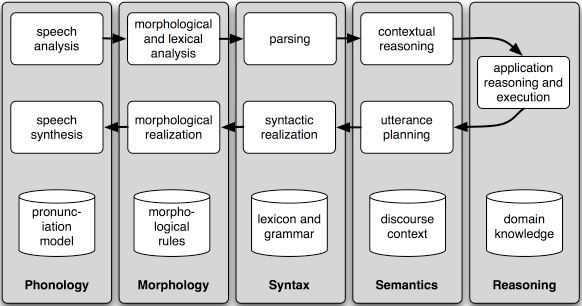
\includegraphics[width=1\textwidth]{pipline}
    \caption{Simple Pipeline Architecture for a Spoken Dialogue System\cite{NLPbook}}
    \label{fig:1}
\end{figure}

In Figure~\ref{fig:1}, \emph{Spoken signal (top left) is taken, speech is recognized, words are parsed and taken in context, application-specific actions occur (top right); a reaction is planned, is realized as a syntactic structure, then to the words that are properly replaced and finally to the spoken output; The different types of linguistic knowledge inform each level of the process.}

Dialogue systems give us the fundamental pipeline for NLP. Figure~\ref{fig:1} 
shows the architecture of a normal dialog system. One of the few language-understanding elements that move left to right at the top of the diagram is "Pipeline". This map is a kind of money-making from the spicinput through the syntactic parsing. In the middle, the opposite pipeline of elements to convert the concept from right to left. These elements create dynamic aspects of the system. Below the diagram there are a few representative organizations of static information: the collection of language-related data for processing materials to do their job.

\subsection{Textual Entailment}
The challenge of language understanding has been brought into focus in recent years by a public "shared task" called Recognizing Textual Entailment (RTE). The basic scenario is simple. Suppose we want to find evidence to support the hypothesis: \emph{Sandra Goudie was defeated by Max Purnell}, and that we have another short text that seems to be relevant, for example, \emph{Sandra Goudie was first elected to Parliament in the 2002 elections, narrowly winning the seat of Coromandel by defeating Labour candidate Max Purnell and pushing incumbent Green MP Jeanette Fitzsimons into third place}. Does the text provide enough evidence for us to accept the hypothesis? In this particular case, the answer will be "No." We can draw this conclusion easily, but it is very hard to come up with automated methods for making the right decision.
Consequently, some linguistic analysis is crucial. In the previous example, it is important for the system to note that \emph{Sandra Goudie} names the person being defeated in the hypothesis, not the person doing the defeating in the text. As another illustration of the difficulty of the task, consider the following text-hypothesis pair:
\begin{enumerate}[a.]
    \item Text: David Golinkin is the editor or author of eighteen books, and over 150 responsa, articles, sermons and books.
    \item Hypothesis: Golinkin has written eighteen books
    
\end{enumerate}

In order to determine whether the hypothesis is supported by the text, the system needs the following background knowledge: (i) if someone is an author of a book, then he/she has written that book; (ii) if someone is an editor of a book, then he/she has not written (all of) that book; (iii) if someone is editor or author of eighteen books, then one cannot conclude that he/she is author of eighteen books.

\subsection{Information Extraction}
With rise of digital age, there is an explosion of information in the form of news, articles, social media, and so on. Much of this data lies in unstructured form and manually managing and effectively making use of it is tedious, boring and labor intensive. This explosion of information and need for more sophisticated and efficient information handling tools gives rise to Information Extraction(IE) and Information Retrieval(IR) technology. Information Extraction systems takes natural language text as input and produces structured information specified by certain criteria, that is relevant to a particular application. Various sub-tasks of IE such as Named Entity Recognition, Coreference Resolution, Named Entity Linking, Relation Extraction, Knowledge Base reasoning forms the building blocks of various high end Natural Language Processing (NLP) tasks such as Machine Translation, Question-Answering System, Natural Language Understanding, Text Summarization and Digital Assistants like Siri, Cortana and Google Now~\cite{DBLP:journals/corr/abs-1807-02383}.
\begin{figure}[htbp]
    \centering
    \includegraphics[width=.8\textwidth]{ie}
    \caption{Simple Pipeline Architecture for an Information Extraction System~\cite{DBLP:journals/corr/abs-1807-02383}.}
    \label{fig:2}
\end{figure}

Figure~\ref{fig:2} shows the architecture for a simple information extraction system. It begins by processing a document using several of the procedures: first, the raw text of the document is split into sentences using a sentence segmenter, and each sentence is further subdivided into words using a tokenizer. Next, each sentence is tagged with part-of-speech tags, which will prove very helpful in the next step, named entity detection. In this step, we search for mentions of potentially interesting entities in each sentence. Finally, we use relation detection to search for likely relations between different entities in the text.
\subsection{Task Definition}
In our project, we are developing an agent that will follow Bengali instructions to navigate in real-life visual environment.
\begin{itemize}
	\item Inputs: Text based instructions in Bengali language.
	\item Outputs: Mapping instructions and visual observations to actions and execute them in the environment.
\end{itemize}

\section{Motivation}
Computers are great at working with structured data like spreadsheets and database tables. But us humans usually communicate in words, not in tables. That’s unfortunate for computers. A lot of information in the world is unstructured raw text in English or another human language. How can we get a computer to understand unstructured text and extract data from it?

Advances in robotics are enabling progressively more sophisticated, capable technologies to reach large consumer populations. Such systems offer unprecedented potential for AI to help in a variety of human-centric applications such as elder care and household maintenance. However, natural, easy-touse interfaces to such systems, such as those employing natural language, are lagging behind. As robots become more prevalent—and as the need for the services they can offer grows—the importance of allowing non-expert users to interact with them naturally and comfortably increases. Natural language is an excellent modality for end users to give instructions and teach robots about their environments~\cite{ijcai2018-810}. 

As long as computers have been around, programmers have been trying to write programs that understand languages like English. The reason is pretty obvious humans have been writing things down for thousands of years and it would be really helpful if a computer could read and understand all that data. 
NLP is important for scientific, economic, social, and cultural reasons. NLP is experiencing rapid growth as its theories and methods are deployed in a variety of new language technologies. For this reason it is important for a wide range of people to have a working knowledge of NLP. Within industry, this includes people in human-computer interaction, business information analysis, and web software development. Within academia, it includes people in areas from humanities computing and corpus linguistics through to computer science and artificial intelligence~\cite{NLPbook}.

\section{Objectives}
By developing the project, we will learn:
\begin{itemize}
    \item To manipulate large corpora, explore linguistic models and analyze language data.
    \item To use the key concepts from NLP and linguistics to describe and analyse language.
    \item To use data structures and linguistics algorithms in robust language processing software.
    \item To extract knowledge from natural language.
    \item To map instructions from natural language to actions.
    \item To deploy an intelligent agent to execute actions in a particular visual environment.
\end{itemize}





